\documentclass[11pt,a4paper]{article}

% Configuración de página y márgenes
\usepackage[margin=1in, top=1.2in, bottom=1.2in]{geometry}

% Paquetes para caracteres especiales y codificación
\usepackage[utf8]{inputenc}
\usepackage[T1]{fontenc}
\usepackage{lmodern}

% Soporte para idiomas (español e inglés)
\usepackage[spanish,english]{babel}

% Paquetes para imágenes y gráficos
\usepackage{graphicx}
\usepackage{float}
\usepackage{caption}
\usepackage{subcaption}

% Paquetes para tablas
\usepackage{longtable}
\usepackage{booktabs}
\usepackage{array}
\usepackage{multirow}
\usepackage{multicol}
\usepackage{tabularx}

% Control de saltos de página
\usepackage{needspace}
\usepackage{afterpage}
\usepackage{placeins}

% Enlaces e hipervínculos
\usepackage[colorlinks=true, linkcolor=blue, urlcolor=blue, citecolor=blue]{hyperref}

% Paquetes para código y verbatim
\usepackage{fancyvrb}
\usepackage{listings}
\usepackage{xcolor}

% Configuración de listings para código
\lstset{
    basicstyle=\ttfamily\small,
    breaklines=true,
    frame=single,
    backgroundcolor=\color{gray!10},
    keywordstyle=\color{blue},
    commentstyle=\color{green!50!black},
    stringstyle=\color{red}
}

% Paquetes para mejor tipografía
\usepackage{microtype}
\usepackage{setspace}

% Configuración de espaciado
\onehalfspacing

% Comandos personalizados
\providecommand{\tightlist}{}

% Comando para evitar viudas y huérfanas
\widowpenalty=10000
\clubpenalty=10000

% Configuración de profundidad de numeración
\setcounter{secnumdepth}{3}
\setcounter{tocdepth}{3}

\begin{document}


    
    % Título principal
    {\Huge \textbf{ICP-10111 Barometric Pressure Sensor}}\\[1.5em]
    
    % Subtítulo si existe
    
    
    % Autor
    
    
    % Fecha
    
    
    \vfill
    
    % Información adicional al pie
    
    
    
\end{titlepage}

% Tabla de contenidos


% Lista de figuras (si hay imágenes)


% Lista de tablas (si hay tablas)




% Contenido principal del documento
\section{Hardware Documentation}

\subsection{Overview}

The ICP-10111 Barometric Pressure Sensor module is a compact embedded sensor with integrated environmental monitoring capabilities, designed for IoT applications and precise atmospheric measurements.

\subsection{Features}

\begin{itemize}
\item \textbf{ICP-10111 Pressure Sensor} (High precision)
\item \textbf{BME688 Environmental Sensor} (Temperature, humidity, gas)
\item \textbf{Low power consumption} modes
\item \textbf{I2C/QWIIC connectivity}
\item \textbf{Compact form factor} with castellated holes
\end{itemize}

\section{Hardware}

\subsection{Technical Specifications Technical Specifications}

\subsubsection{Sensor Specifications}


\begin{table}[H]
\centering
\small
\begin{tabular}{|l|l|l|l|}
\hline
Parameter & Value & Unit & Notes \\
\hline
Pressure Range & 300-1250 & hPa & Absolute pressure \\
Pressure Accuracy & $\pm$0.4 & hPa & At 25$^{\circ}$C \\
Temperature Range & -40 to +85 & $^{\circ}$C & Operating range \\
Humidity Range & 0-100 & %RH & Relative humidity \\
Interface & I2C & - & QWIIC compatible \\
\hline
\end{tabular}
\caption{Especificaciones técnicas}
\end{table}


\subsubsection{Power Specifications}


\begin{table}[H]
\centering
\small
\begin{tabular}{|l|l|l|l|l|l|}
\hline
Parameter & Min & Typ & Max & Unit & Conditions \\
\hline
Supply Voltage & 3.0 & 3.3 & 5.0 & V & Normal Operation \\
Active Current & - & 1.2 & 2.0 & mA & Continuous measurement \\
Sleep Current & - & 0.1 & 0.5 & $\mu$A & Standby mode \\
Regulator Output & - & 1.8 & - & V & Internal LDO \\
\hline
\end{tabular}
\caption{Especificaciones técnicas}
\end{table}


\subsection{Pinout Pinout}


\begin{figure}[H]
\centering
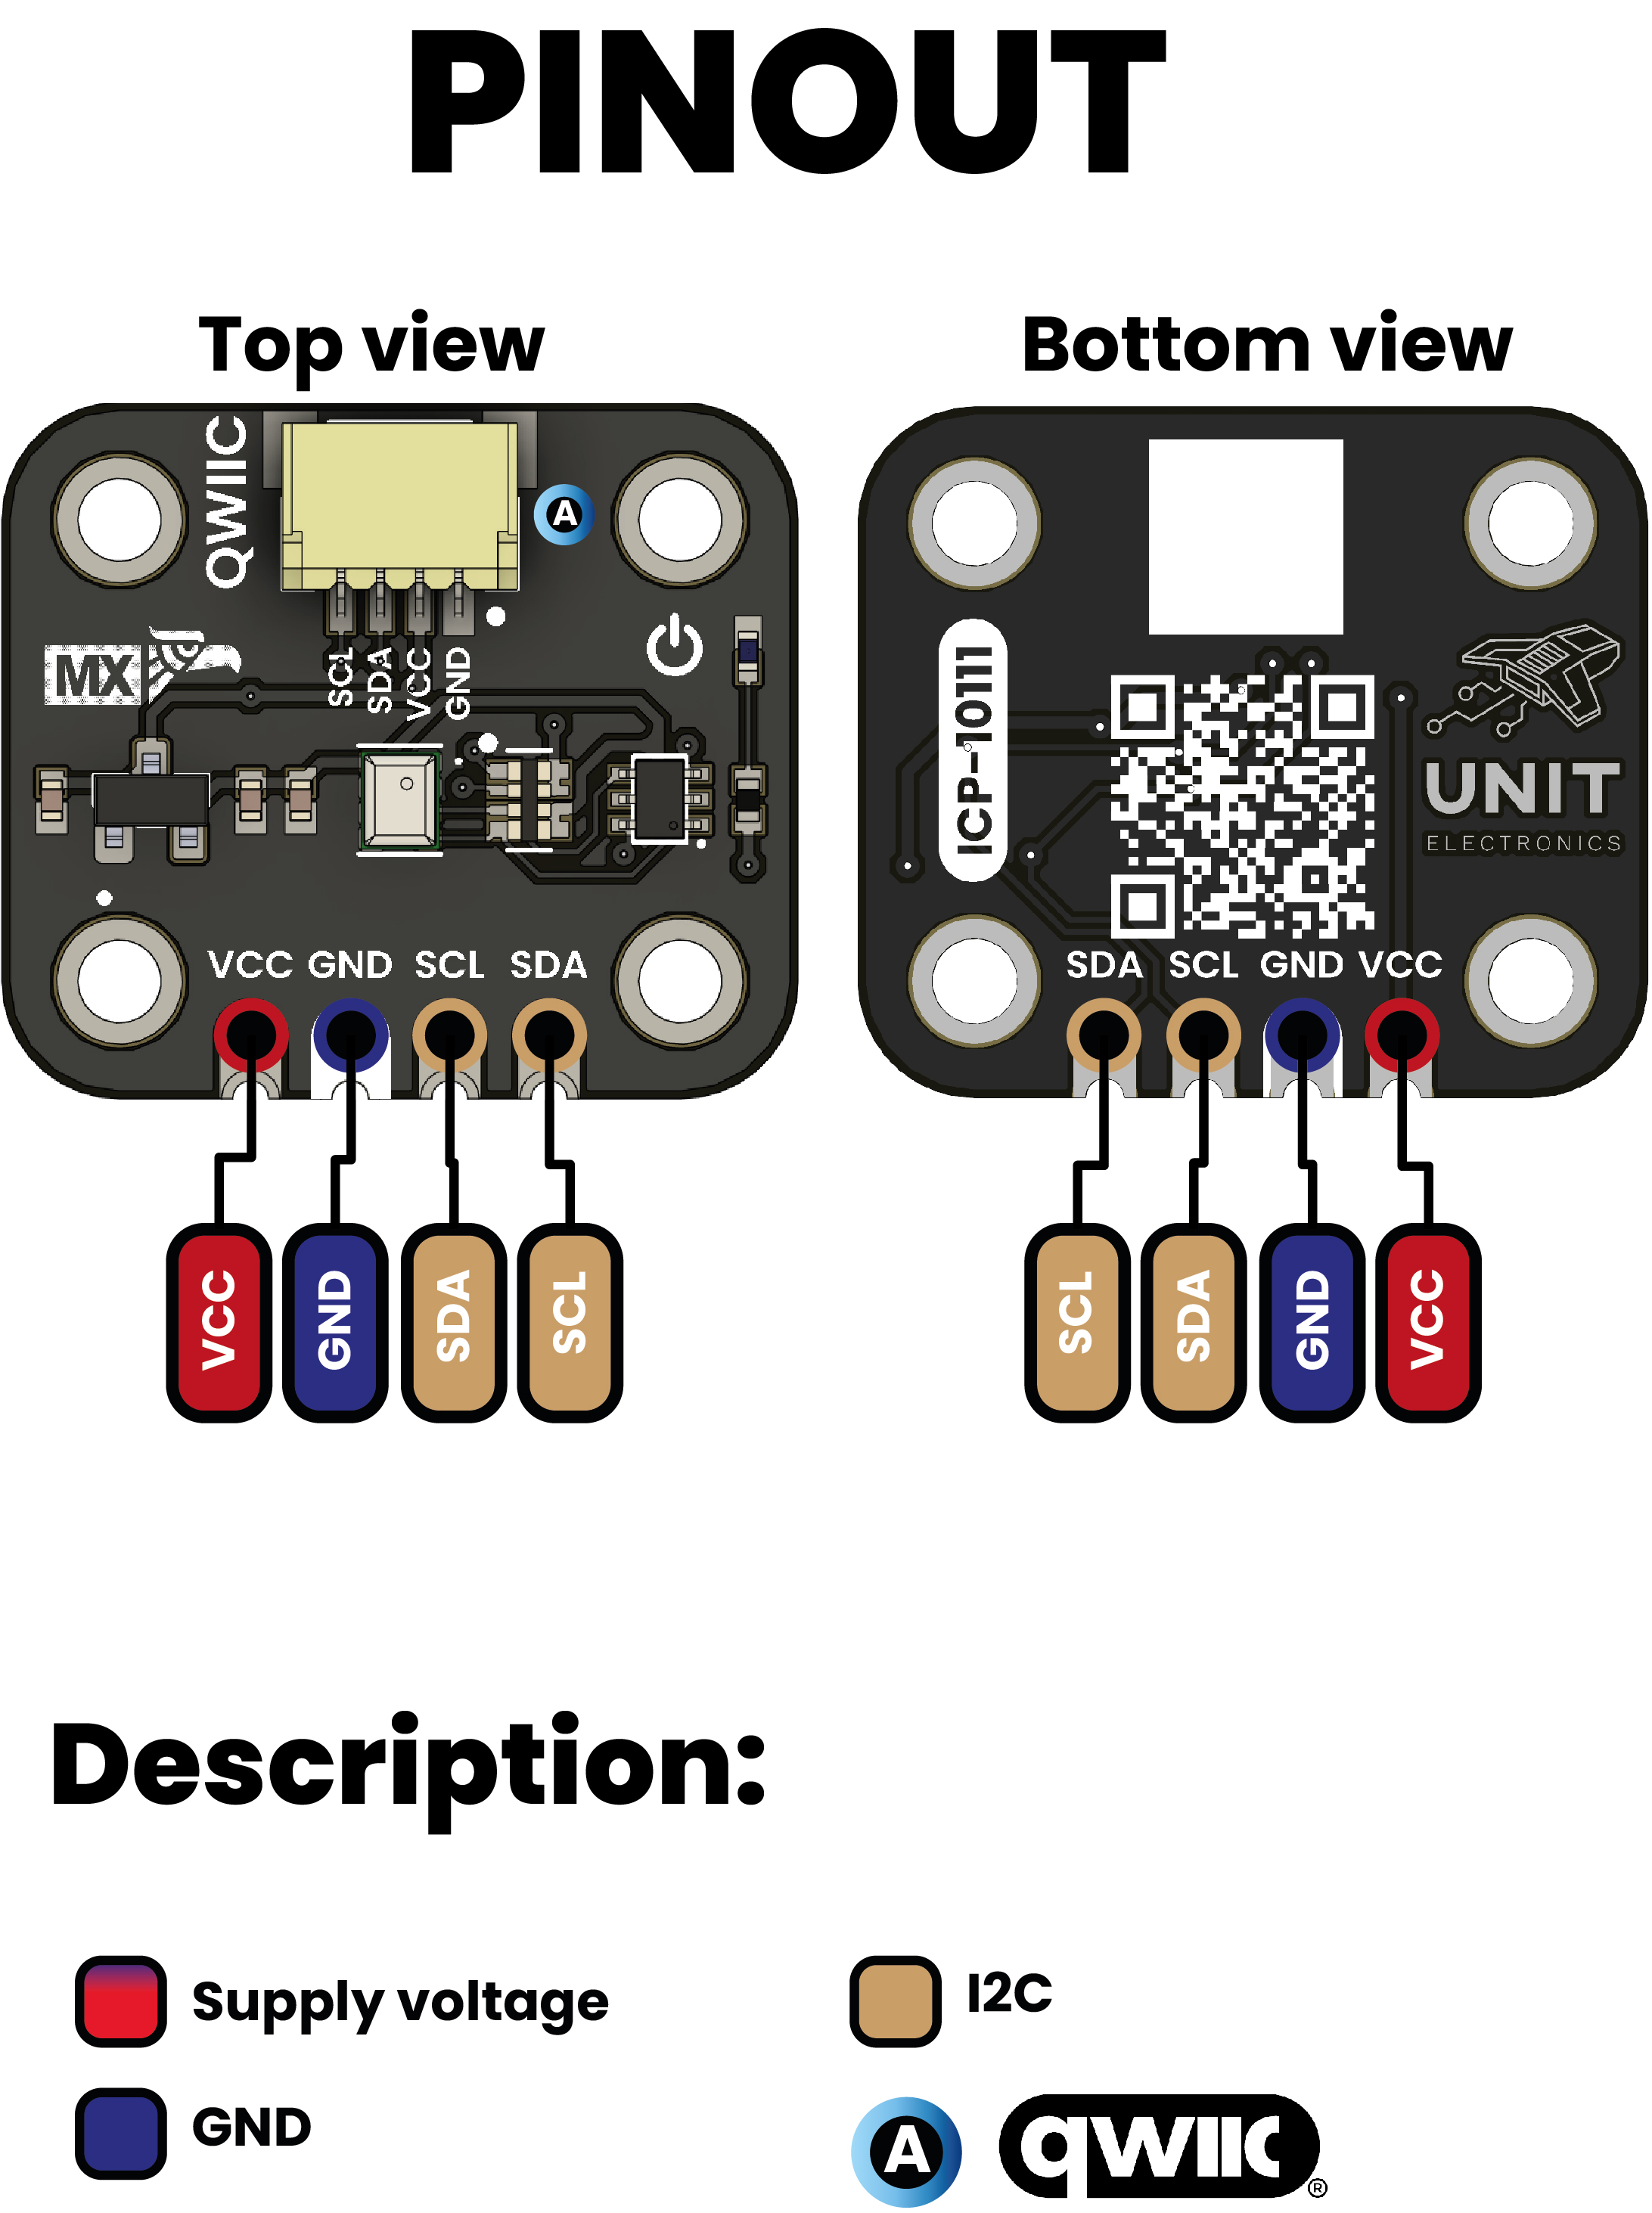
\includegraphics[width=0.9\textwidth]{en_unit_pinout_v_0_0_1_ue0094_icp10111_barometric_pressure_sensor_en.jpg}
\caption{Pinout Diagram}
\label{fig:en-unit-pinout-v-0-0-1-ue0094-icp10111-barometric-pressure-sensor-en-jpg}
\end{figure}




\begin{table}[H]
\centering
\small
\begin{tabular}{|c|c|c|}
\hline
Pin Label & Function & Notes \\
\hline
VCC & Power Supply & 3.3V or 5V \\
GND & Ground & Common ground for all components \\
SDA & I2C Data & Serial data line \\
SCL & I2C Clock & Serial clock line \\
\hline
\end{tabular}
\caption{Especificaciones técnicas}
\end{table}


\subsection{Dimensions Dimensions}


\begin{figure}[H]
\centering
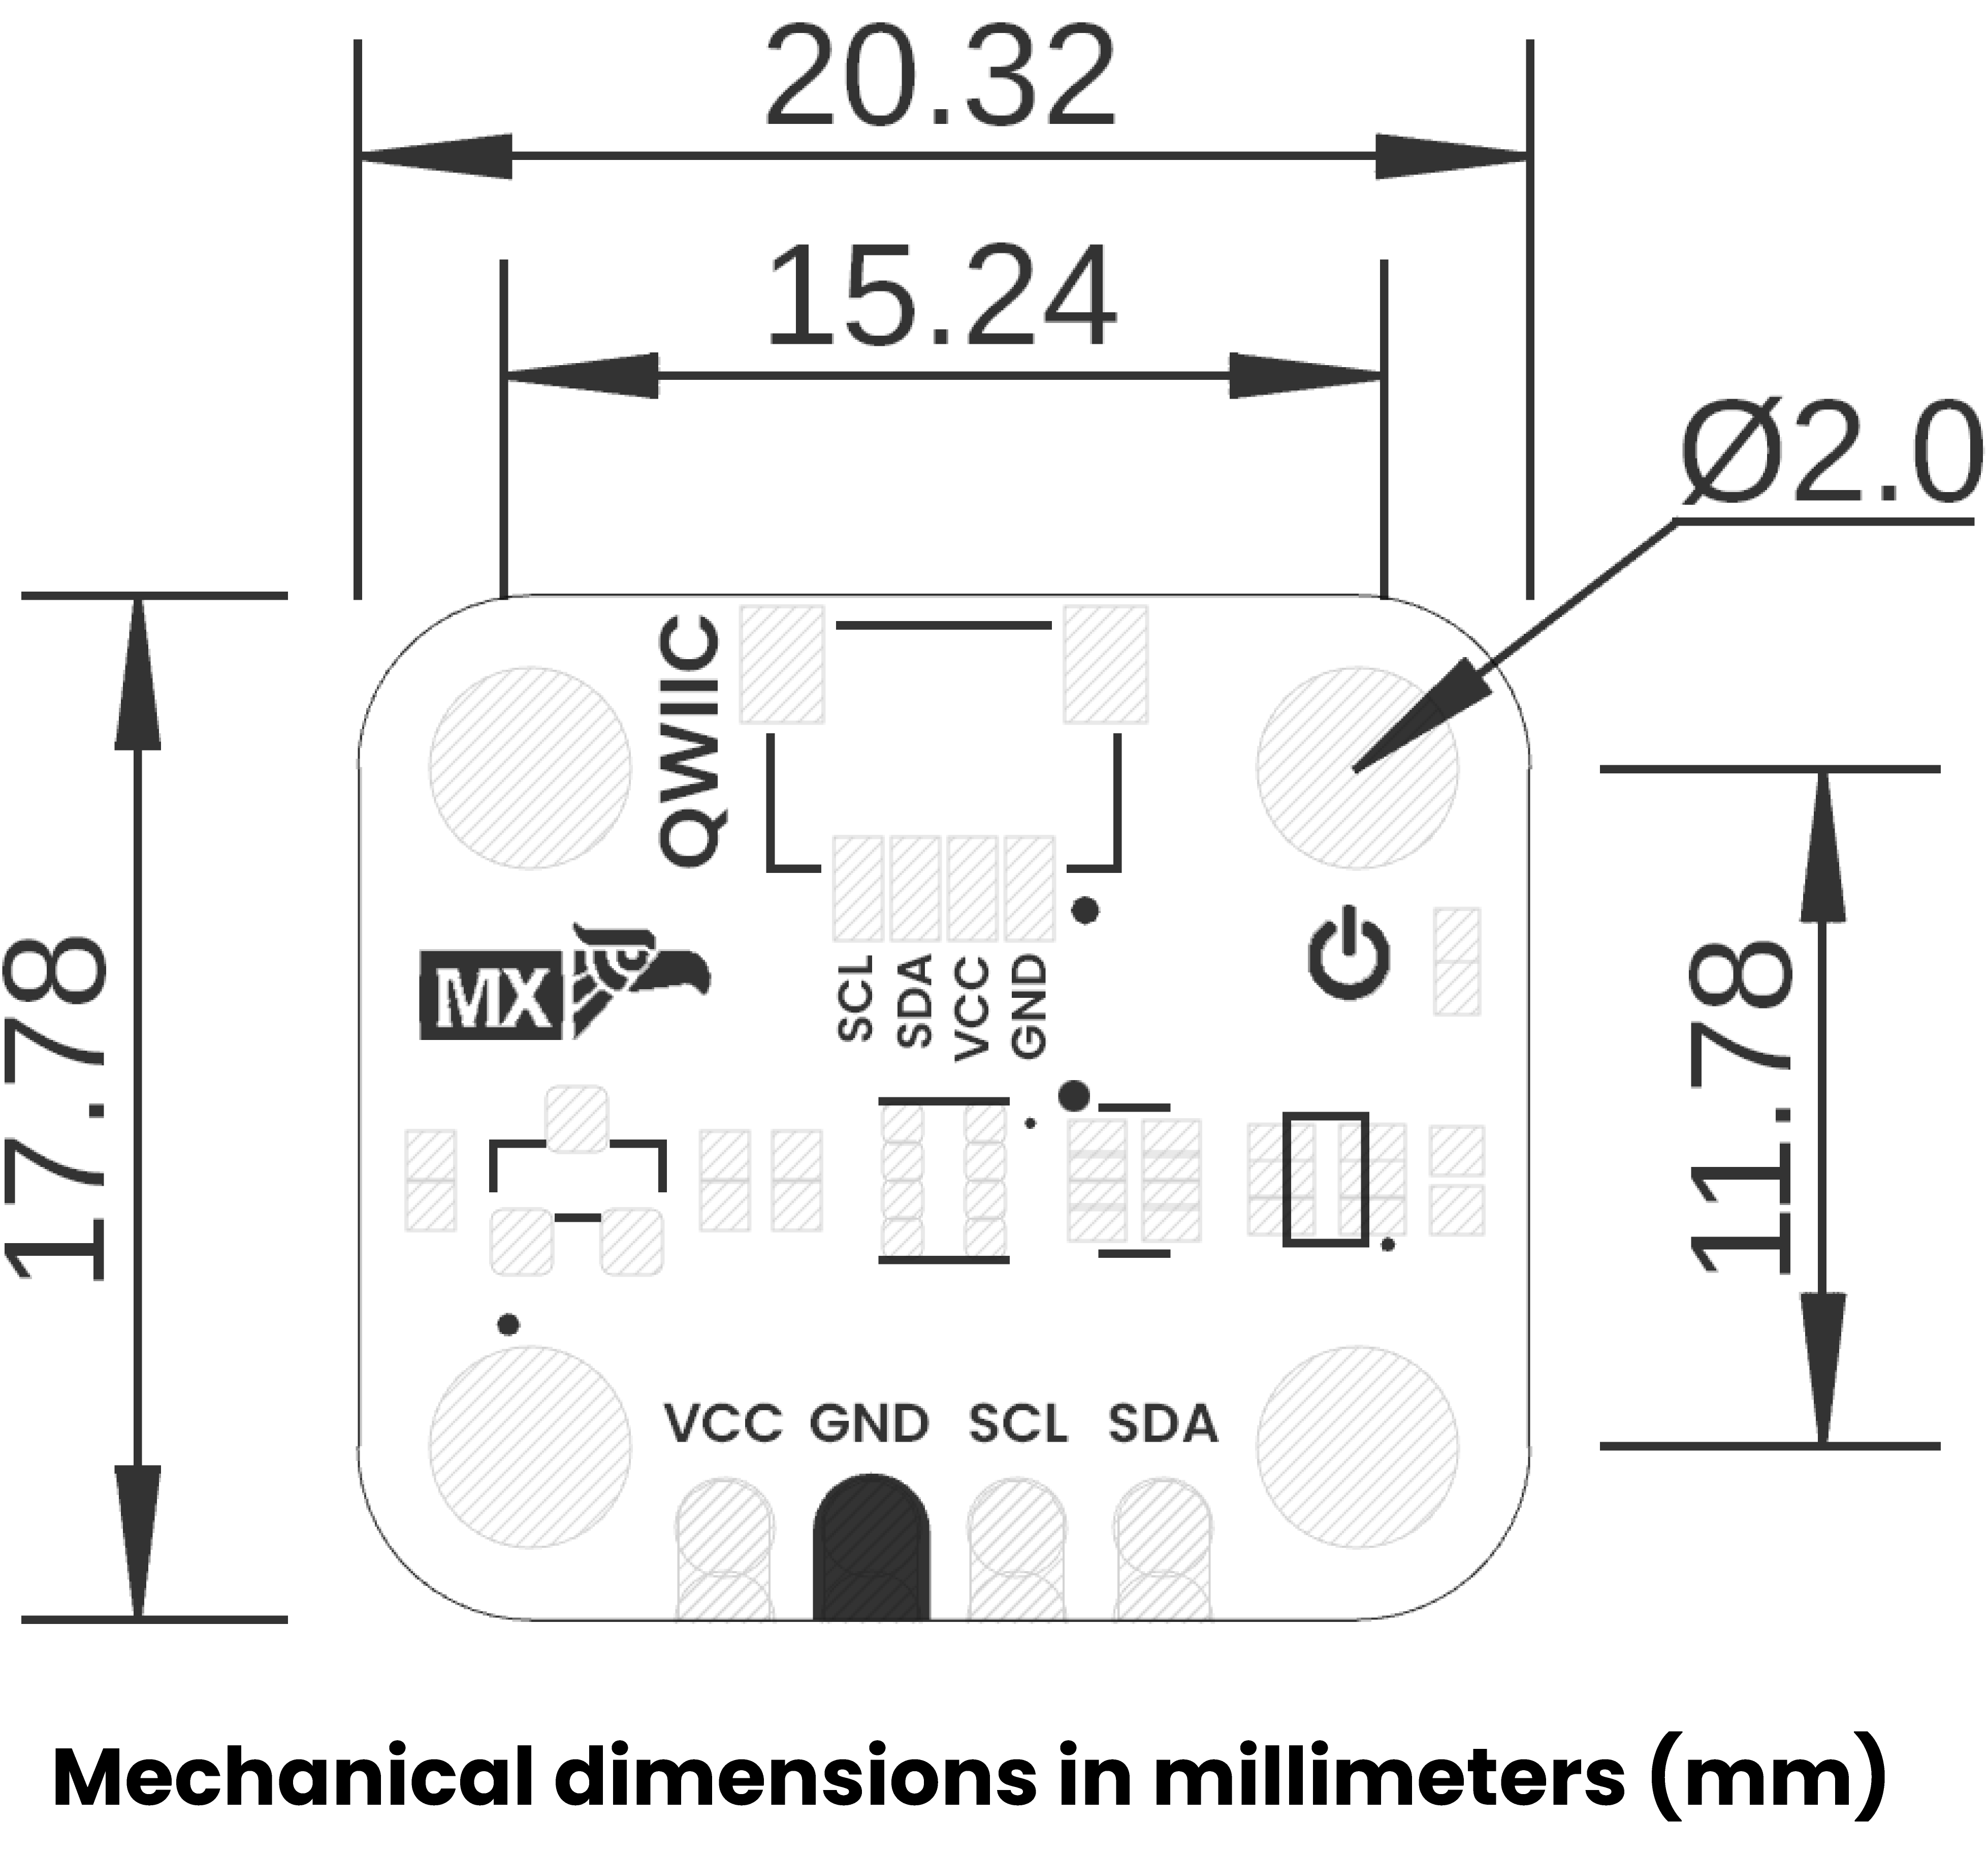
\includegraphics[width=0.6\textwidth]{en_unit_dimension_v_1_0_0_icp10111_barometric_pressure_sensor.png}
\caption{Dimensions}
\label{fig:en-unit-dimension-v-1-0-0-icp10111-barometric-pressure-sensor-png}
\end{figure}



\subsection{Topology Topology}


\begin{figure}[H]
\centering
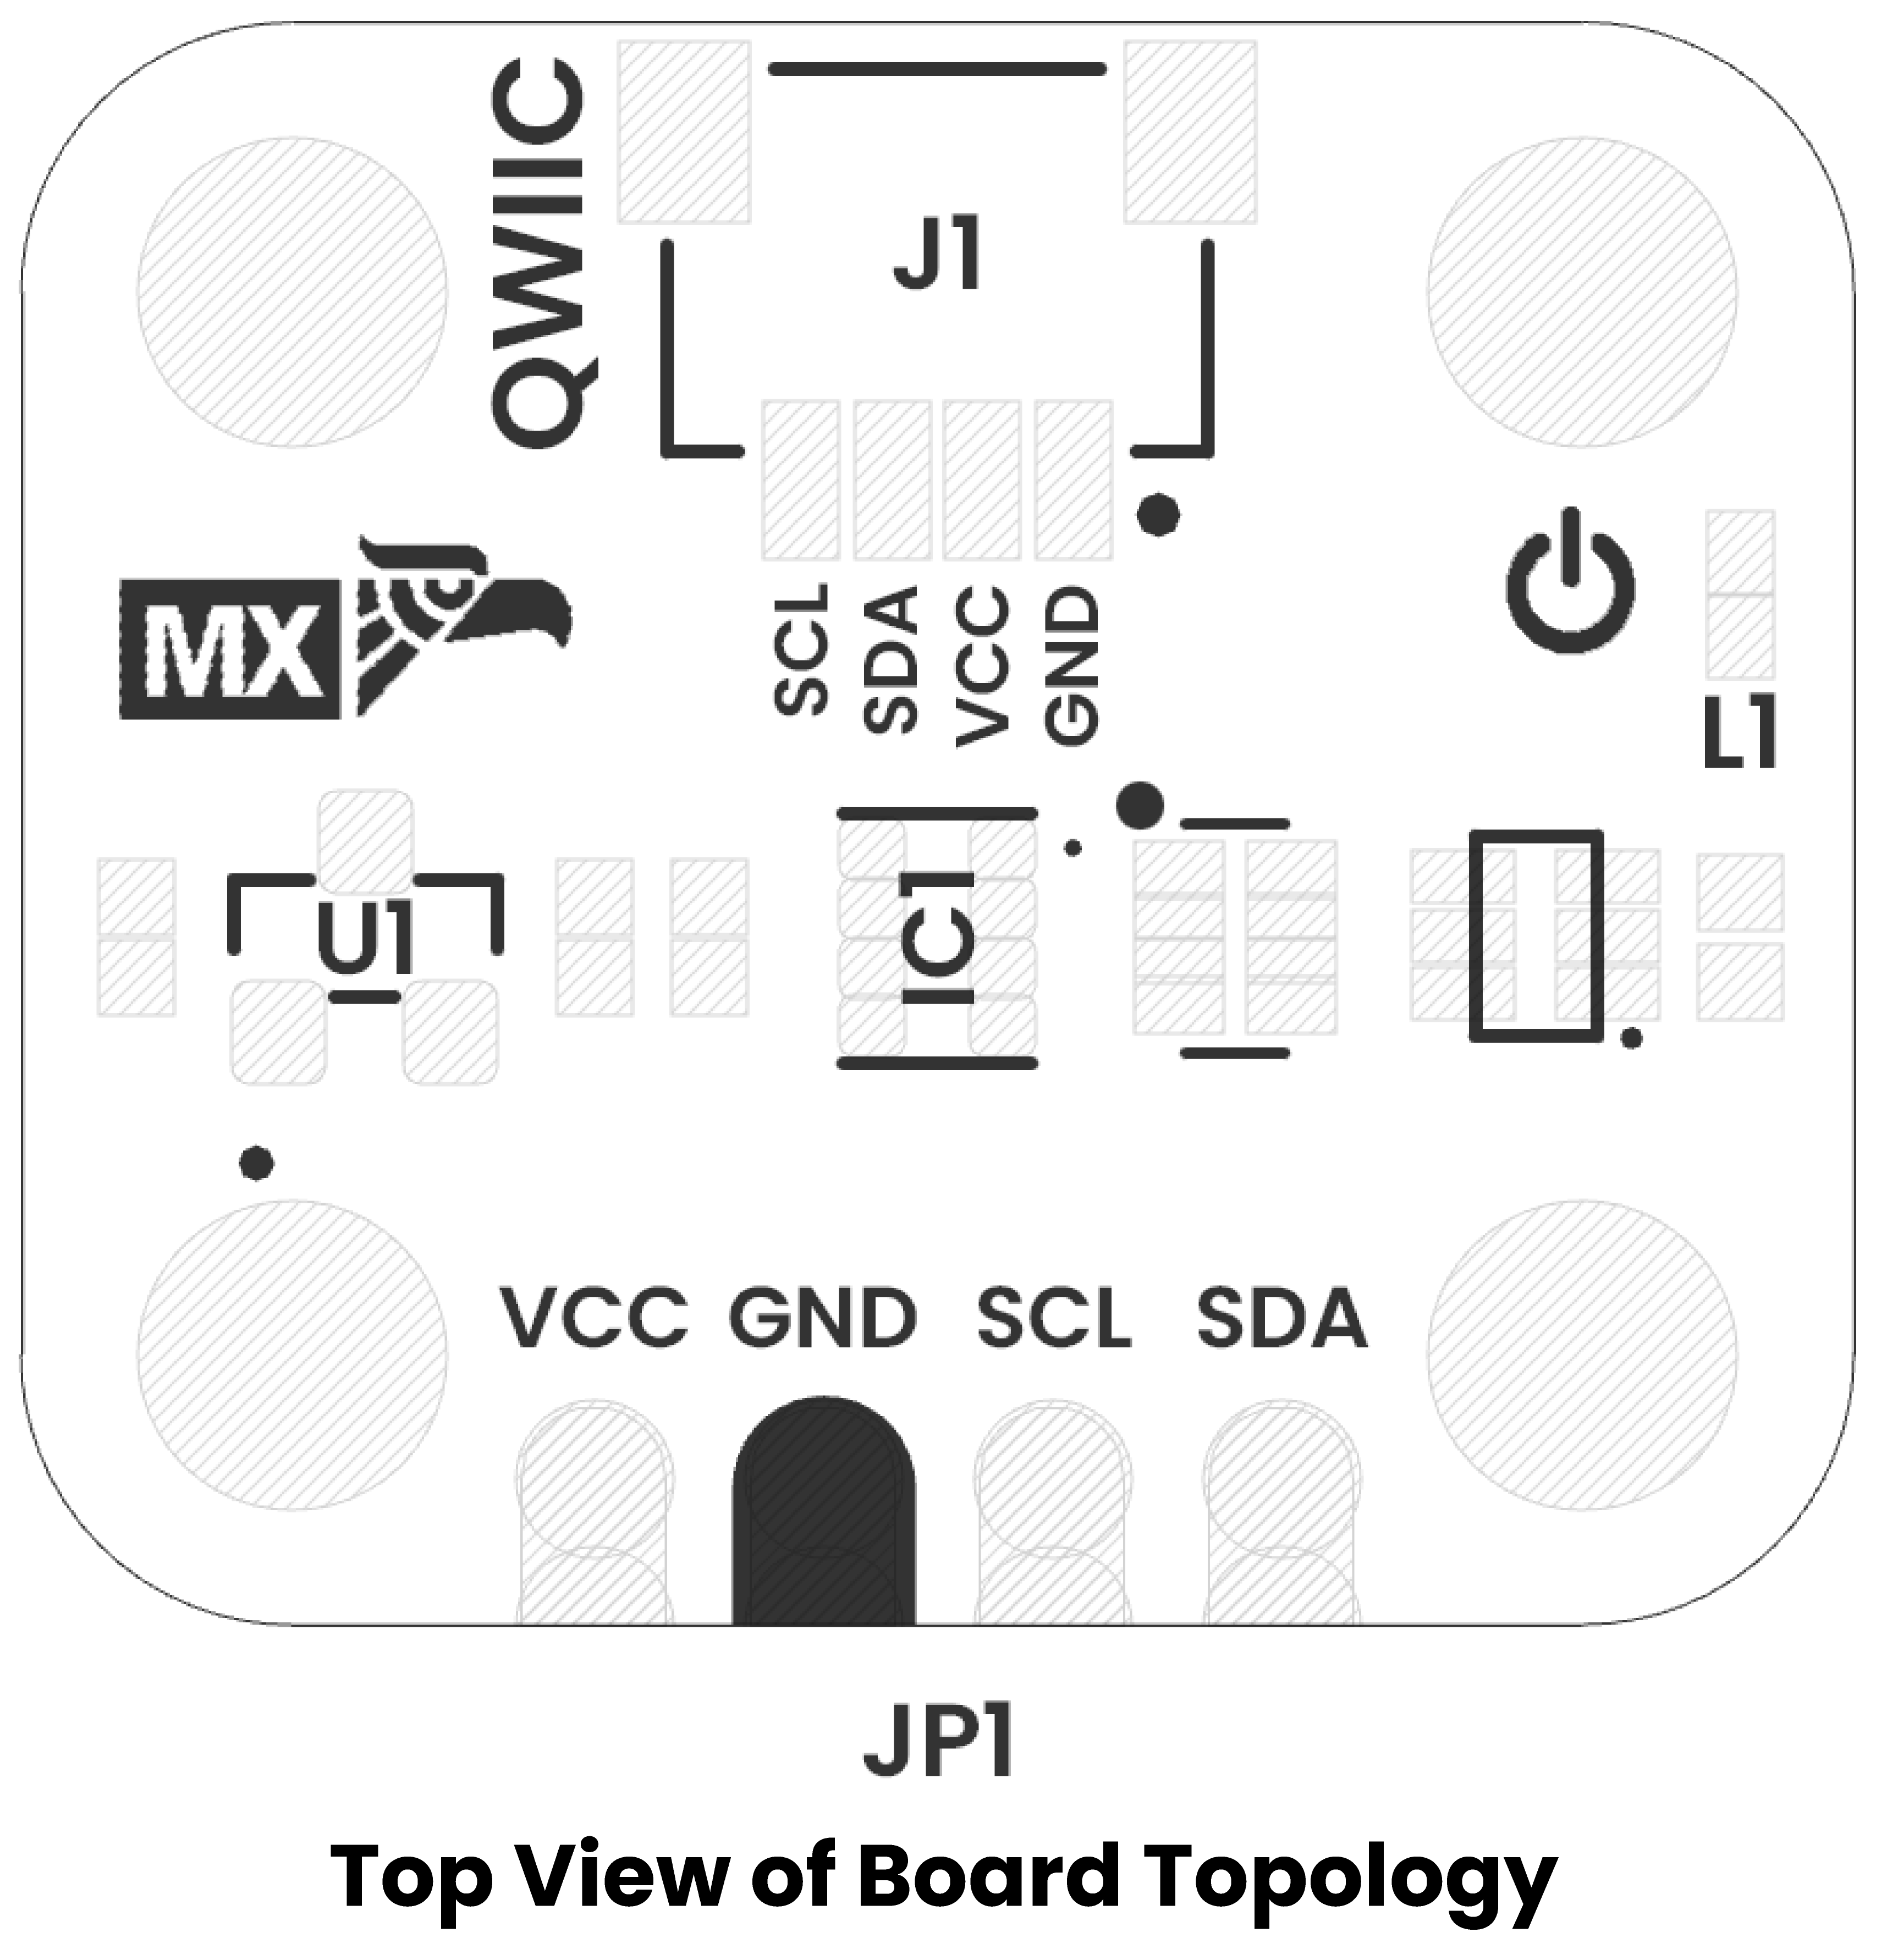
\includegraphics[width=0.7\textwidth]{en_unit_topology_v_1_0_0_icp10111_barometric_pressure_sensor.png}
\caption{Topology}
\label{fig:en-unit-topology-v-1-0-0-icp10111-barometric-pressure-sensor-png}
\end{figure}




\begin{table}[H]
\centering
\small
\begin{tabular}{|c|c|}
\hline
Ref. & Description \\
\hline
IC1 & ICP-10111 Barometric Pressure Sensor \\
IC2 & BME688 Environmental Sensor \\
L1 & Power On LED \\
U1 & ME6206A18XG 1.8V Regulator \\
JP1 & 2.54 mm Castellated Holes \\
J1 & QWIIC Connector (JST 1 mm pitch) for I2C \\
\hline
\end{tabular}
\caption{Especificaciones técnicas}
\end{table}


\subsection{Communication Interfaces}

\subsubsection{I2C Interface}
\begin{itemize}
\item \textbf{Address}: 0x63 (ICP-10111), 0x77 (BME688)
\item \textbf{Speed}: Standard (100 kHz), Fast (400 kHz)
\item \textbf{Features}: QWIIC compatible connector
\item \textbf{Pull-up Resistors}: 4.7k$\Omega$ integrated
\end{itemize}

\subsubsection{Digital Interface Specifications}
\begin{itemize}
\item \textbf{Logic Levels}: 3.3V CMOS compatible
\item \textbf{Input High}: 2.0V minimum
\item \textbf{Input Low}: 0.8V maximum
\item \textbf{Output Drive}: 4mA typical
\end{itemize}

\subsection{Physical Characteristics}

\subsubsection{Package Information}


\begin{table}[H]
\centering
\small
\begin{tabular}{|c|c|c|}
\hline
Parameter & Value & Unit \\
\hline
Package Type & Custom PCB & - \\
Dimensions & 25.4 x 15.24 x 3.2 & mm \\
Mounting & Castellated holes & 2.54mm pitch \\
Weight & 2.1 & g \\
\hline
\end{tabular}
\caption{Especificaciones técnicas}
\end{table}


\subsubsection{Environmental Specifications}


\begin{table}[H]
\centering
\small
\begin{tabular}{|l|l|l|l|l|}
\hline
Parameter & Min & Max & Unit & Conditions \\
\hline
Operating Temperature & -40 & +85 & $^{\circ}$C & Full accuracy \\
Storage Temperature & -55 & +125 & $^{\circ}$C & - \\
Humidity & 0 & 100 & %RH & Non-condensing \\
Pressure Range & 300 & 1250 & hPa & Absolute pressure \\
\hline
\end{tabular}
\caption{Especificaciones técnicas}
\end{table}


\subsection{Software Support}

\subsubsection{Development Environment}
\begin{itemize}
\item \textbf{Arduino IDE}: Full library support
\item \textbf{ESP-IDF}: Native driver integration
\item \textbf{PlatformIO}: Cross-platform support
\item \textbf{CircuitPython}: Python library available
\end{itemize}

\subsubsection{Key Libraries}
\begin{itemize}
\item ICP-10111 pressure sensor driver
\item BME688 environmental sensor library
\item I2C communication protocols
\item Data filtering and calibration
\end{itemize}

\subsection{Applications}

The ICP-10111 module is ideal for:

\begin{enumerate}
\item \textbf{Weather Monitoring}
\end{enumerate}
\begin{itemize}
\item Atmospheric pressure measurement
\item Altitude determination
\item Weather prediction systems
\end{itemize}

\begin{enumerate}
\item \textbf{IoT Environmental Sensing}
\end{enumerate}
\begin{itemize}
\item Smart building automation
\item Agricultural monitoring
\item Air quality assessment
\end{itemize}

\begin{enumerate}
\item \textbf{Portable Devices}
\end{enumerate}
\begin{itemize}
\item Fitness trackers
\item Outdoor navigation devices
\item Drone altitude control
\end{itemize}

\subsection{Safety and Compliance}

\subsubsection{Certifications}
\begin{itemize}
\item \textbf{RoHS}: Compliant with EU directive
\item \textbf{REACH}: Compliant with EU regulation
\item \textbf{CE}: Electromagnetic compatibility
\end{itemize}

\subsubsection{Safety Features}
\begin{itemize}
\item \textbf{ESD Protection}: $\pm$2kV HBM on all pins
\item \textbf{Reverse Polarity Protection}: Integrated
\item \textbf{Thermal Protection}: Operating range monitoring
\end{itemize}

\subsection{References}

\begin{itemize}
\item \href{https://product.tdk.com/system/files/dam/doc/product/sensor/pressure/capacitive-pressure/data_sheet/ds-000177-icp-10111-v1.3.pdf}{ICP-10111 Datasheet}
\item \href{https://www.bosch-sensortec.com/media/boschsensortec/downloads/datasheets/bst-bme688-ds000.pdf}{BME688 Datasheet}
\item \href{https://www.microne.com.cn/uploads/file/20200904/ME6206.pdf}{ME6206 Regulator Datasheet}
\end{itemize}

\subsection{Ordering Information}


\begin{table}[H]
\centering
\small
\begin{tabular}{|l|l|l|l|}
\hline
Part Number & Description & Package & MOQ \\
\hline
ICP10111-001 & Standard Module & Individual & 1 \\
ICP10111-DEV & Development Kit & Kit Box & 1 \\
ICP10111-BULK & Bulk Order & Tray & 100 \\
\hline
\end{tabular}
\caption{Especificaciones técnicas}
\end{table}


\subsection{Revision History}


\begin{table}[H]
\centering
\small
\begin{tabular}{|c|c|c|}
\hline
Version & Date & Changes \\
\hline
1.0 & 2025-07-18 & Initial release \\
\hline
\end{tabular}
\caption{Especificaciones técnicas}
\end{table}


\subsection{Schematics}


\begin{figure}[H]
\centering
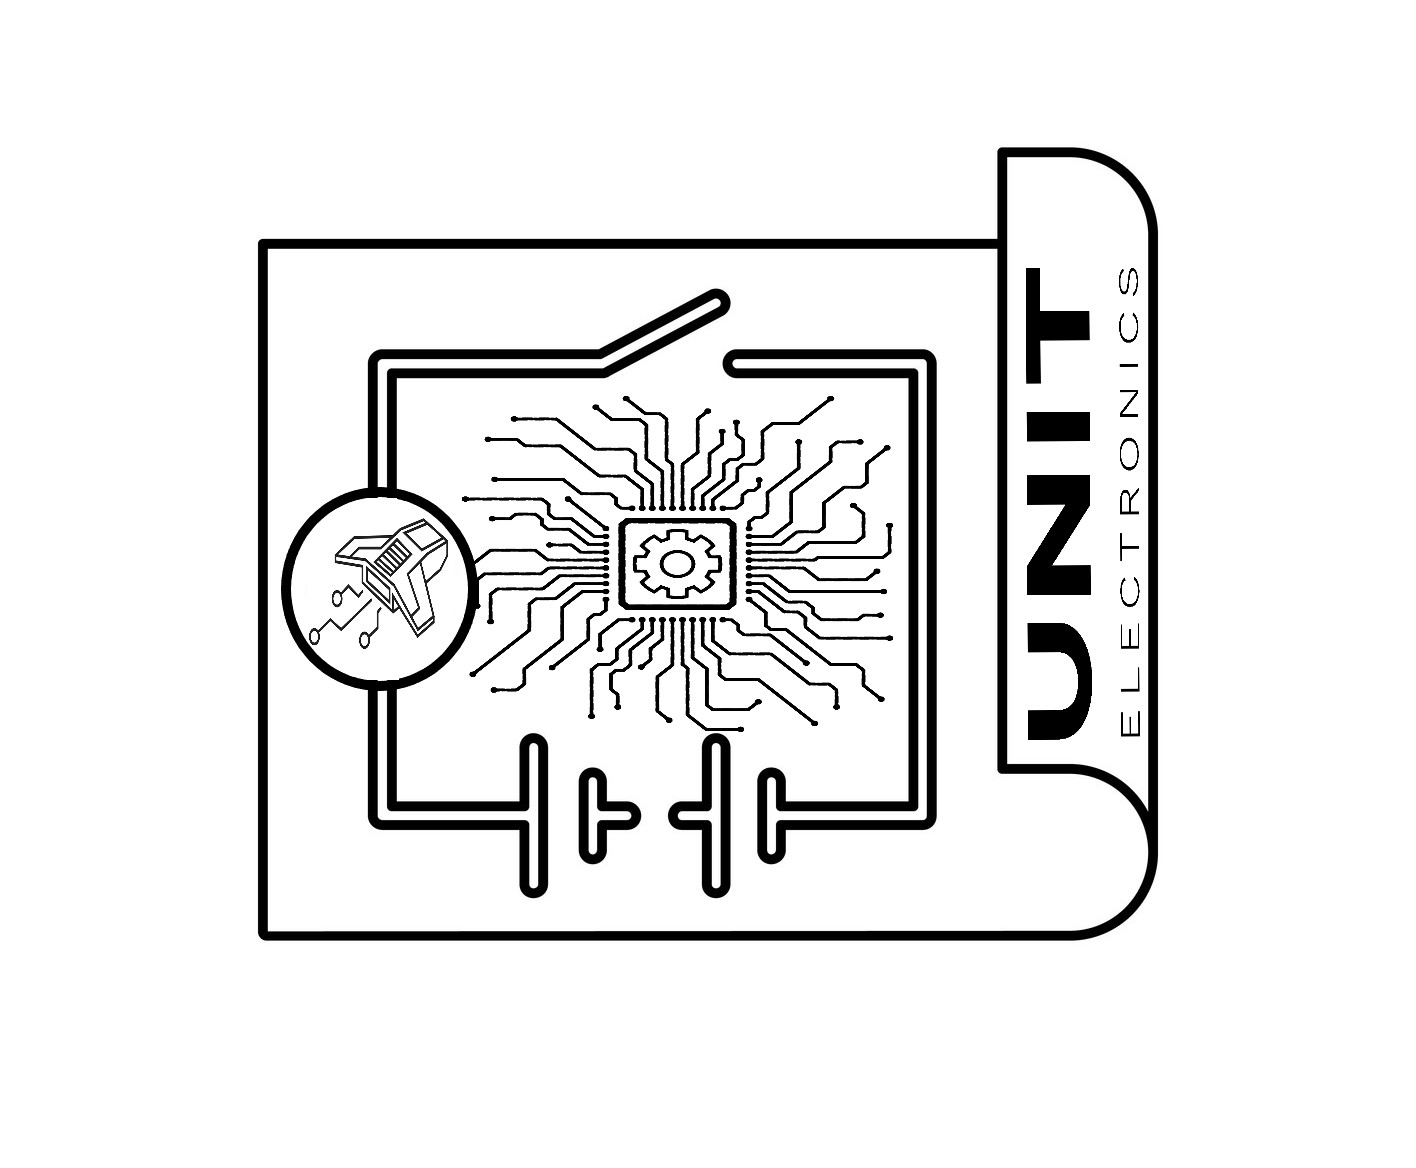
\includegraphics[width=\textwidth]{en_Schematics_icon.jpg}
\caption{Circuit Schematic}
\label{fig:en-Schematics-icon-jpg}
\end{figure}



---

\textit{For technical support and additional information, visit our website or contact our engineering team.}


\end{document}
